% ==============================================================
% Kuantum Fiziği -- ana kitap dosyası
% ÖNERİLEN DERLEME: latexmk -pdf book.tex
% (latexmk Biber adımını otomatik çalıştırır.)
% Ana kitap için bu dosyayı derleyin: book.tex
%
% Her bölüm aynı zamanda bağımsız derlenebilir:
%   01nciBolum.tex
%   02nciBolum.tex
% vb.
% ==============================================================

\documentclass[a4paper,12pt,twoside]{article}

% --------------------------------------------------------------
% ORTAK AYARLAR
% Bütün bölüm dosyaları bu preamble'ı subfiles aracılığıyla
% miras alır. Böylece ayarlar tek yerde tutulur.
% --------------------------------------------------------------
\usepackage[
  papersize={210mm,297mm},
  tmargin=20mm,
  bmargin=20mm,
  lmargin=20mm,
  rmargin=20mm
]{geometry}

\usepackage[utf8]{inputenc}
\usepackage[T1]{fontenc}
\usepackage{lmodern}
%%\usepackage{textcomp}
\usepackage[english,turkish,shorthands=off]{babel}
\usepackage{csquotes}

\usepackage{amsmath,amssymb,mathabx}
\usepackage{siunitx}
\usepackage{lscape}
\usepackage{tcolorbox}
\usepackage{enumitem}

\usepackage{hyperref}
\hypersetup{
  colorlinks,
  citecolor=black,
  filecolor=black,
  linkcolor=blue,
  urlcolor=red
}

\usepackage{graphicx}
\graphicspath{{./figurler/}{./kapaklar/}}

\usepackage[colorinlistoftodos]{todonotes}
\usepackage{fancyhdr}
\usepackage{indentfirst}
\setlength{\parindent}{5ex}
\setlength{\headheight}{15pt}
\usepackage{pdfpages}

% Bölümlerin hem bağımsız hem de book.tex içinde çalışmasını sağlar.
\usepackage{subfiles}

% Denklem numaralrını her bölümde yeniden başlatmak için
\usepackage{chngcntr}
\counterwithin{equation}{section}
\counterwithin{figure}{section}
\counterwithin{table}{section}

% --------------------------------------------------------------
% KAYNAKÇA
% Tek veri tabanı, her bölüm için ayrı refsection.
% Backend BIBER'dır (BibTeX değil).
% --------------------------------------------------------------
%\usepackage[
%  backend=biber,
%  style=numeric,
%  sorting=nyt,
%  giveninits=true
%]{biblatex}

\usepackage[
backend=biber,
style=numeric,
sorting=none,
giveninits=true,
doi=false,
isbn=false,
url=true
]{biblatex}


\addbibresource{kuantum.bib}

% Her bölümün kaynakçası, o bölümün section başlığının altında
% bir subsection düzeyinde görünür ve ortak içindekilere eklenir.
\defbibheading{chapterbibliography}{%
  \subsection*{Kaynaklar}%
  \addcontentsline{toc}{subsection}{Kaynaklar}%
}

% Bir bölüm tek başına derleniyorsa kendi refsection'ını açıp kapatır.
% Aynı dosya book.tex içinden çağrıldığında refsection'ı ana dosya yönetir.
\newcommand{\printbib}{
	
	\vspace{36pt}
	\setquotestyle{english}
	\printbibliography[heading=chapterbibliography]%
	}

\newcommand{\BolumKaynakcaBaslat}{%
  \ifSubfilesClassLoaded{
  	\tableofcontents
  	\listoffigures
  	\listoftables
  	\clearpage
  	
  	\begin{refsection}
  	}{}%
}
\newcommand{\BolumKaynakcaBitir}{%
  \ifSubfilesClassLoaded{%
    %%\clearpage
    
    \printbib
    \end{refsection}%
  }{}%
}

\newcommand{\YAZILACAK}{{\vspace{18pt}\bfseries\Large\color{red} YAZILACAK}}

% --------------------------------------------------------------
% Üst / alt bilgi
% --------------------------------------------------------------
\pagestyle{fancy}
\fancyhf{}
\lhead{Kuantum Fiziği}
\chead{\thepage}
\rhead{Mesut Karakoç}
\lfoot{Akdeniz Üniversitesi}
\cfoot{}

\title{Akdeniz Üniversitesi\\ Fen Fakültesi - Fizik Bölümü\\FİZ319 Kuantum Fiziği Ders Notları}
\author{Prof. Dr. Mesut Karakoç}
\date{\today}

\renewcommand{\contentsname}{İçindekiler}

% ==============================================================
\begin{document}
% ==============================================================

% --------------------------------------------------------------
% KAPAK
% --------------------------------------------------------------
\IfFileExists{kapaklar/kapak.pdf}{%
  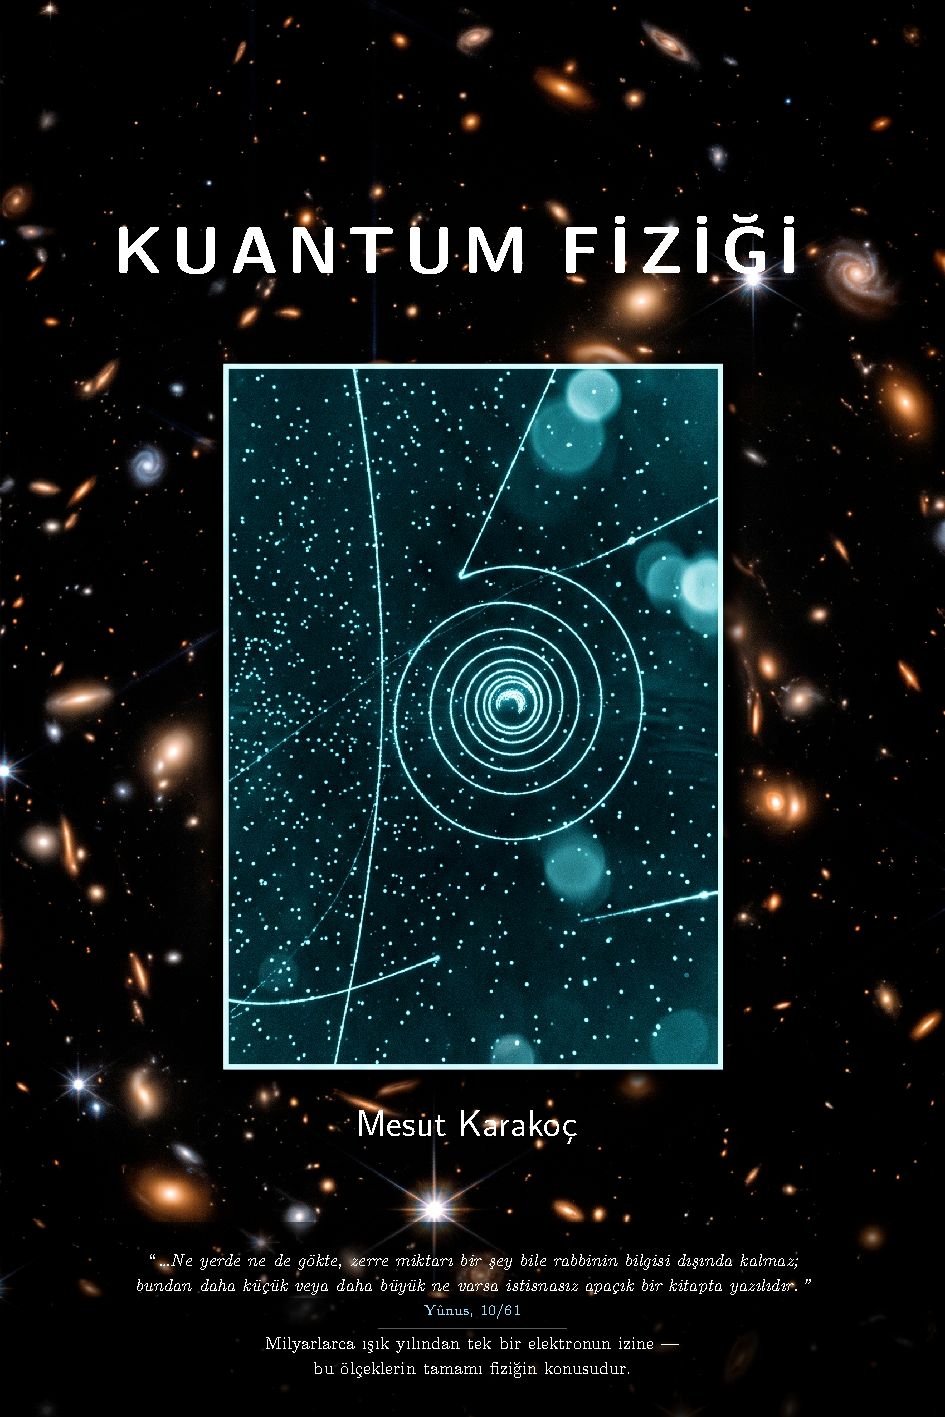
\includepdf[
    pages=1,
    fitpaper=false,
    width=\paperwidth,
    height=\paperheight,
    pagecommand={\thispagestyle{empty}}
  ]{kapaklar/kapak.pdf}%
}{%
  % Kapak henüz yoksa kitap yine derlenebilsin.
  \begin{titlepage}
    \centering
    \vspace*{0.22\textheight}
    {\Huge\bfseries Kuantum Fiziği\par}
    \vspace{2cm}
    {\Large Prof. Dr. Mesut Karakoç\par}
    \vfill
    {\large Akdeniz Üniversitesi\par}
  \end{titlepage}
}

\setcounter{page}{1}
\clearpage

% --------------------------------------------------------------
% ORTAK İÇİNDEKİLER / ŞEKİLLER / TABLOLAR
% --------------------------------------------------------------
\tableofcontents
\listoffigures
\listoftables
\clearpage

% --------------------------------------------------------------
% BÖLÜMLER
% Ana kitapta her bölüm kendi refsection'ı içinde tutulur.
% Böylece her bölümün kaynakçası yalnızca o bölümde atıf yapılan
% kaynaklardan oluşur. Bölüm dosyalarının kendileri de bağımsız
% derlenebilir (bkz. \BolumKaynakcaBaslat / \BolumKaynakcaBitir).
% --------------------------------------------------------------
\begin{refsection}
  \subfile{01nciBolum.tex}
  %%\clearpage
  
  \printbib
\end{refsection}

\clearpage
\begin{refsection}
  \subfile{02nciBolum.tex}
  %%\clearpage
  
  \printbib
\end{refsection}

\clearpage
\begin{refsection}
  \subfile{03ncuBolum.tex}
  %%\clearpage

\printbib
\end{refsection}

\clearpage
\begin{refsection}
	\subfile{04ncuBolum.tex}
	%%\clearpage
	
	\printbib
\end{refsection}


\end{document}
